\documentclass[10pt, compress, aspectratio=169]{beamer}

\usetheme[numbering=none, progressbar=none, titleformat=smallcaps, sectionpage=none]{metropolis}

\usepackage{sourcecodepro}
\usepackage{booktabs}
\usepackage{array}
\usepackage{listings}
\usepackage{graphicx}
\usepackage{import}
\usepackage[english]{babel}
\usepackage[scale=2]{ccicons}
\usepackage{url}
\usepackage{relsize}
\usepackage{wasysym}

\usepackage{pgfplots}
\usepgfplotslibrary{dateplot}

\definecolor{Base}{HTML}{191F26}
\definecolor{Accent}{HTML}{157FFF}

\setbeamercolor{alerted text}{fg=Accent}
\setbeamercolor{frametitle}{bg=Base}

\setsansfont[BoldFont={Source Sans Pro Semibold},
              Numbers={OldStyle}]{Source Sans Pro}

\lstset{ %
  backgroundcolor={},
  basicstyle=\ttfamily\footnotesize,
  breakatwhitespace=true,
  breaklines=true,
  captionpos=n,
  commentstyle=\color{orange},
  escapeinside={\%*}{*)},
  extendedchars=true,
  frame=n,
  keywordstyle=\color{Accent},
  language=C++,
  rulecolor=\color{black},
  showspaces=false,
  showstringspaces=false,
  showtabs=false,
  stepnumber=2,
  stringstyle=\color{gray},
  tabsize=2,
  keywords={thrust,plus,device_vector, copy,transform,begin,end, copyin,
  copyout, acc, \_\_global\_\_, void, int, float, main, threadIdx, blockIdx,
  blockDim, if, else, malloc, NULL, cudaMalloc, cudaMemcpy, cudaSuccess,
  cudaGetLastError, cudaDeviceSynchronize, cudaFree, cudaMemcpyDeviceToHost,
  cudaMemcpyHostToDevice, const, data, independent, kernels, loop,
  fprintf, stderr, cudaGetErrorString, EXIT_FAILURE, for, dim3},
  otherkeywords={::, \#pragma, \#include, <<<,>>>, \&, \*, +, -, /, [, ], >, <}
}

\renewcommand*{\UrlFont}{\ttfamily\smaller\relax}

\graphicspath{{../img/}}

\title{Autotuning for High Performance Computing}
\author{\footnotesize Pedro Bruel \\ {\scriptsize \emph{phrb@ime.usp.br}}}
\institute{
\includegraphics[height=2cm]{imelogo}\\[0.2cm] Instituto de Matemática e Estatística \\ Universidade de São Paulo}
\date{\scriptsize \today}

\begin{document}

%\maketitle

%\section*{Introduction}
%
%\subsection*{About}
%
%\begin{frame}
%    \frametitle{About}
%    \begin{columns}[T,onlytextwidth]
%        \column{0.5\textwidth}
%        \begin{center}
%            
\includegraphics[width=.32\textwidth]{pedro}
%
%            Pedro Bruel
%
%            \textit{phrb@ime.usp.br}
%        \end{center}
%
%        \begin{center}
%            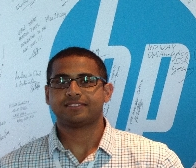
\includegraphics[width=.34\textwidth]{sai}
%
%            Sai Rahul Chalamalasetti
%
%            \textit{sairahul.chalamalasetti@hpe.com}
%        \end{center}
%
%        \column{0.5\textwidth}
%        \begin{center}
%            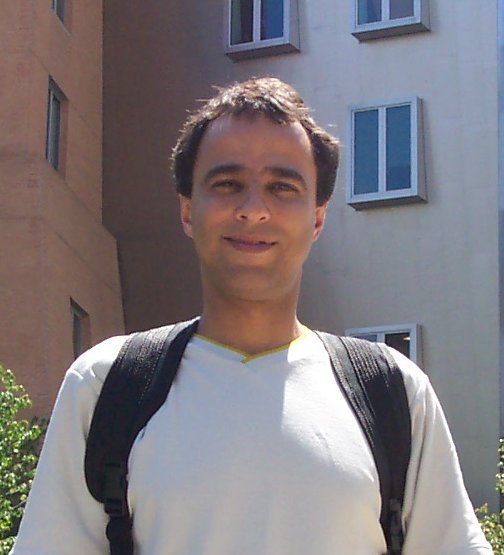
\includegraphics[width=.3\textwidth]{alfredo}
%
%            Alfredo Goldman
%
%            \textit{gold@ime.usp.br}
%        \end{center}
%
%        \begin{center}
%            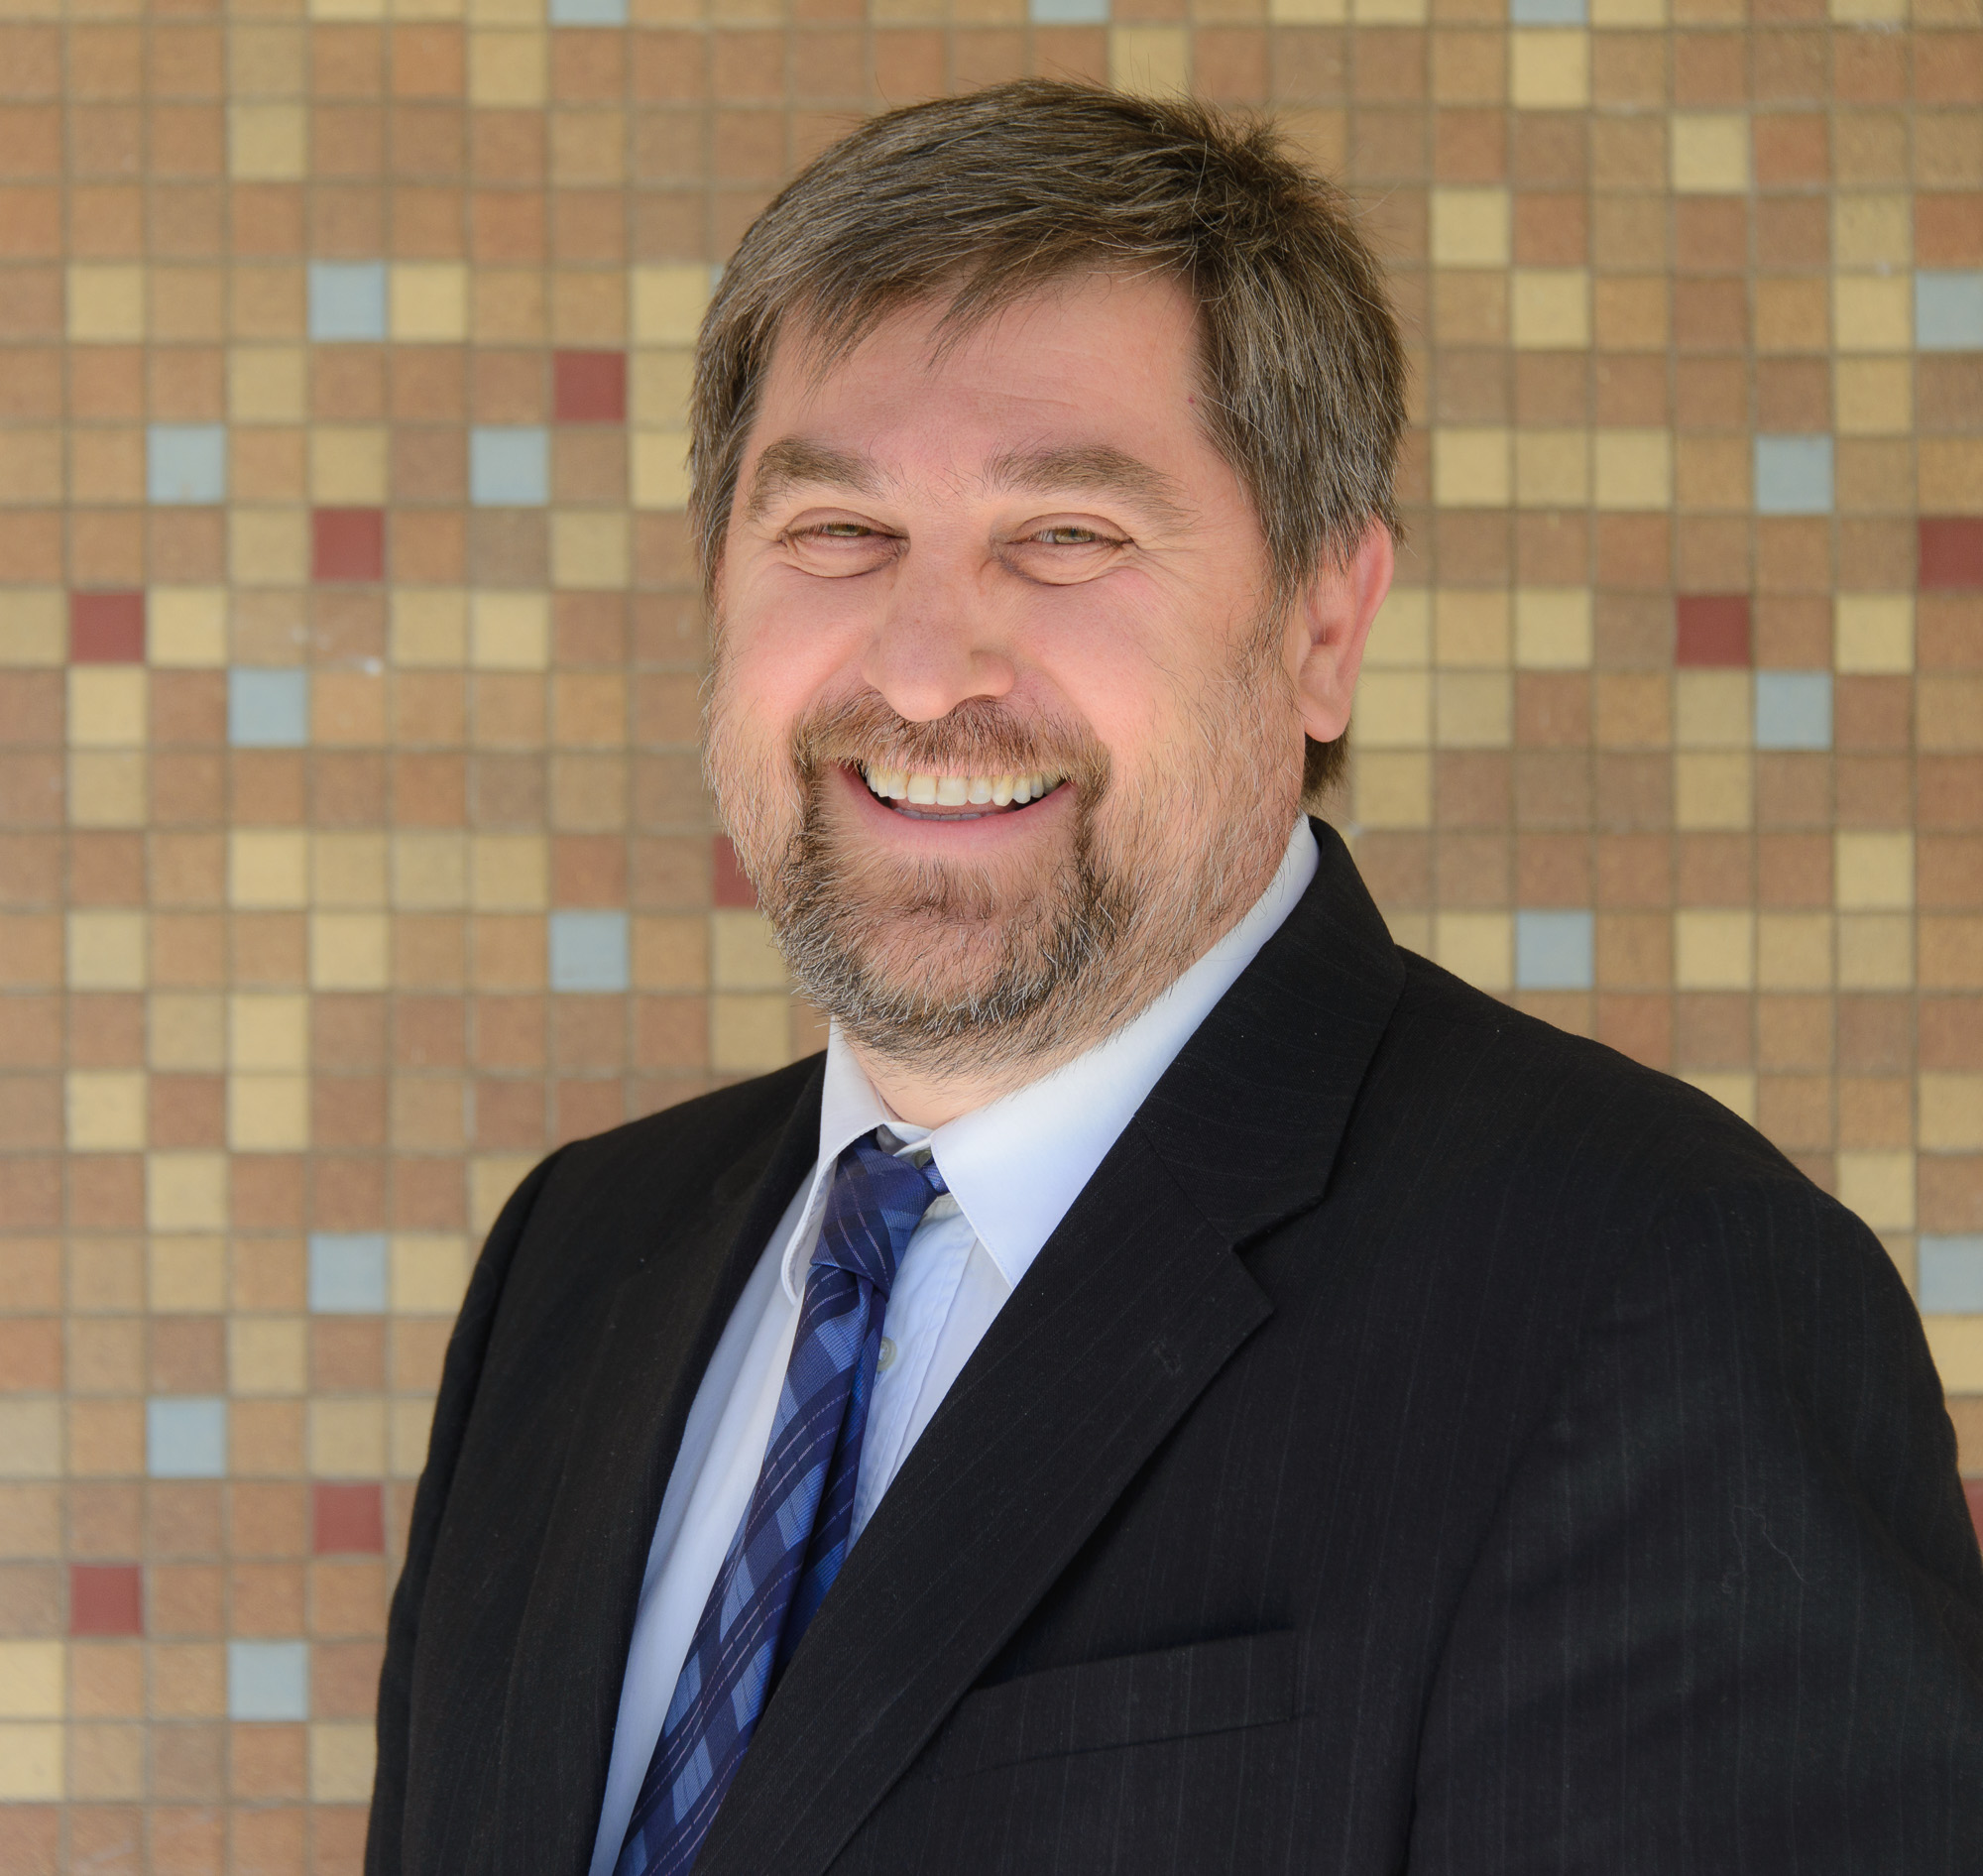
\includegraphics[width=.32\textwidth]{dejan}
%
%            Dejan Milojicic
%
%            \textit{dejan.milojicic@hpe.com}
%        \end{center}
%
%    \end{columns}
%\end{frame}
%
%\subsection*{Outline}
%
%\begin{frame}
%    \frametitle{Outline}
%    \setbeamertemplate{section in toc}[sections numbered]
%    \tableofcontents[hideallsubsections]
%\end{frame}

\section{Autotuning}

\begin{frame}
    \frametitle{Autotuning: Optimization as a Search Problem}
    Casting program optimization as a \alert{search problem}:

    \begin{columns}[T,onlytextwidth]
        \column{0.5\textwidth}
        \alert{Search Spaces}:
        \begin{itemize}
            \item Algorithm Selections
            \item Program Configurations
            \item $\dots$
        \end{itemize}

        \column{0.5\textwidth}
        \alert{Search Objectives}:
        \begin{itemize}
            \item Minimize \alert{execution time}
            \item Maximize \alert{usage of resources}
            \item $\dots$
        \end{itemize}
    \end{columns}

    \vfill
\end{frame}

%\begin{frame}
%    \frametitle{Search Spaces \& Techniques}
%    The \alert{search spaces} created by program optimization problems can be
%    \alert{difficult to explore}
%
%    \begin{center}
%        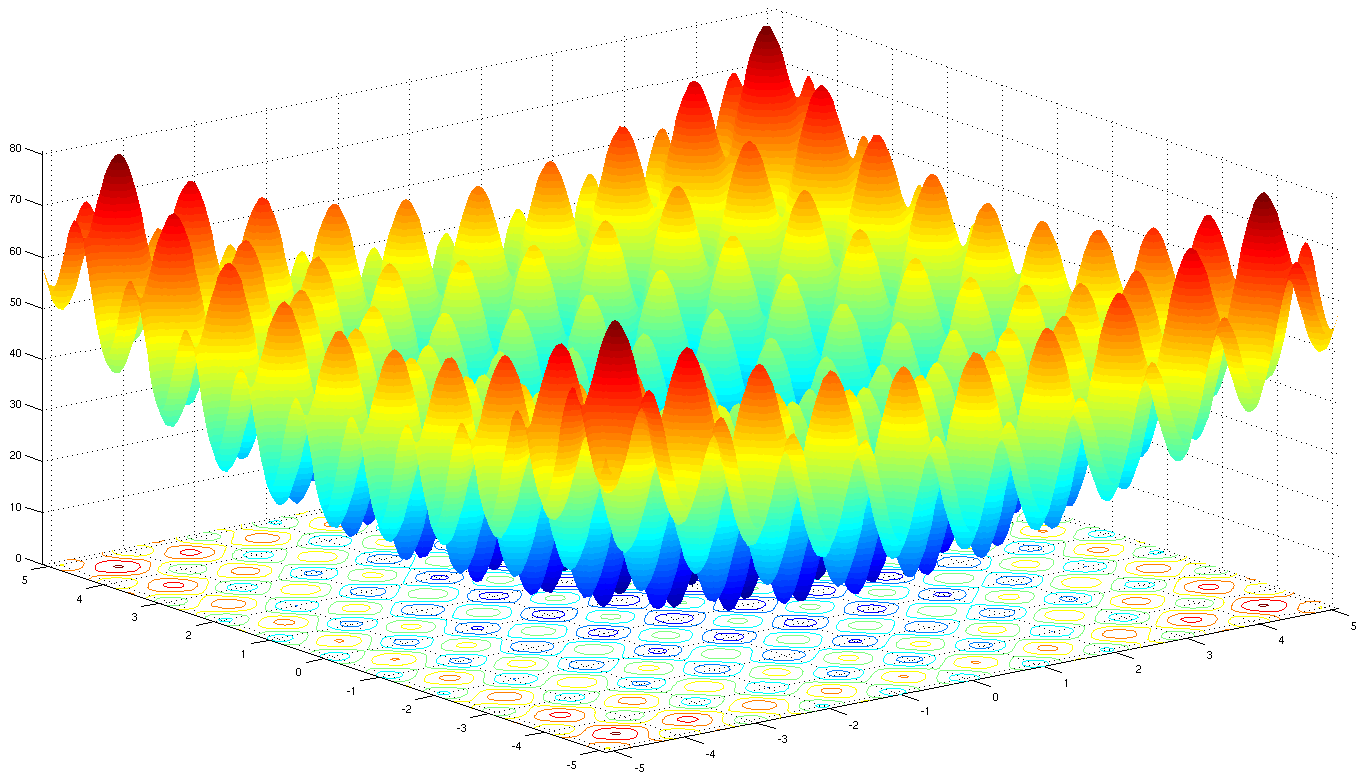
\includegraphics[width=.6\textwidth]{rastrigin}
%
%        Rastrigin function, with \alert{global minimum} $f(0,0) = 0$
%    \end{center}
%\end{frame}

\begin{frame}
    \frametitle{Search Spaces \& Techniques}
    \begin{table}[]
        \centering
        \begin{tabular}{@{}ccc@{}}
            \toprule
            System & Domain & Technique \\ \midrule
            ATLAS & Dense Linear Algebra & Exhaustive \\
            Insieme & Compiler & Genetic Algorithm \\
            SPIRAL & DSP Algorithms & Pareto Active Learning \\
            Active Harmony & Runtime & Nelder-Mead \\ \bottomrule
        \end{tabular}
        \caption{Some autotuning systems, their domains and techniques}
    \end{table}

    \begin{itemize}
        \item Different \alert{problem domains} generate different \alert{search spaces}
        \item \alert{No single solution} for all domains
        \item Search techniques can be composed: \alert{OpenTuner}
        \item Independent searches can be \alert{parallelized and distributed}
    \end{itemize}
\end{frame}

%\begin{frame}
%    \frametitle{Autotuning: Abstract Model}
%    \begin{center}
%        
\includegraphics[width=.5\textwidth]{overview}
%    \end{center}
%\end{frame}

\section{Autotuning GPU Compiler Parameters}

\begin{frame}
    \frametitle{NVIDIA CUDA Compiler: From CUDA C++ to Object Code}
    \begin{center}
        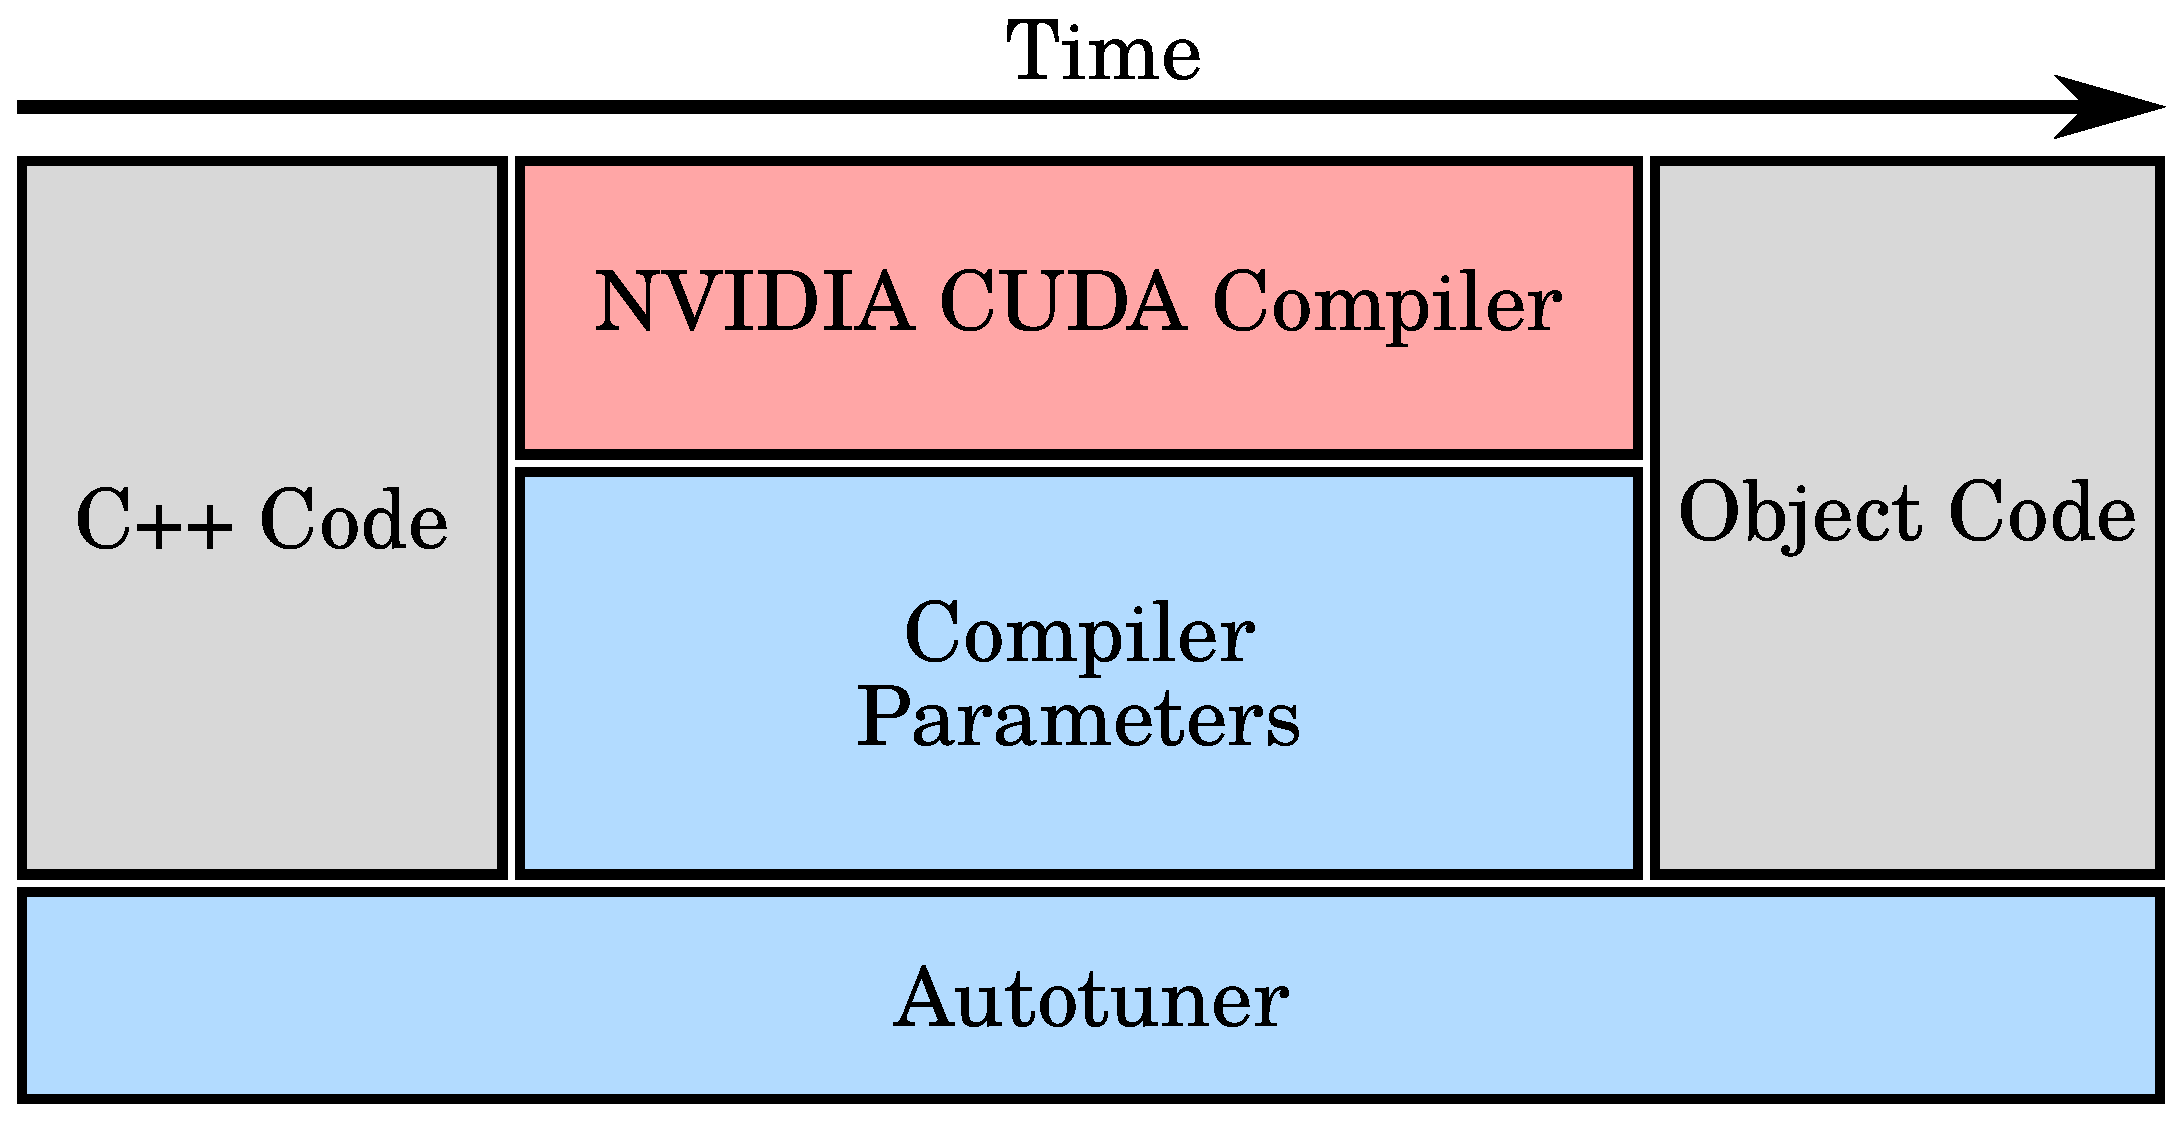
\includegraphics[width=.6\textwidth]{gpu-stack}
    \end{center}

    \begin{itemize}
        \item We tuned applications from the \alert{Rodinia Benchmark Suite}
        \item C++ $\rightarrow$ Object Code: takes \alert{seconds}; \alert{up to 4x speedup}
        \item We \alert{tuned the parameters} of the NVIDIA CUDA Compiler (NVCC)
    \end{itemize}
\end{frame}

%\begin{frame}
%    \frametitle{Autotuning: GPUs}
%    \begin{center}
%        
\includegraphics[width=.73\textwidth]{overview_gpus}
%
%        \alert{1h} of tuning $\rightarrow \; \dfrac{3600s}{\sim{}s} \approx \alert{10^3}$ \alert{iterations}
%    \end{center}
%\end{frame}

\begin{frame}
    \frametitle{Results}
    \alert{Most significative speedups} for \alert{Rodinia applications}
    and \alert{matrix multiplication optimizations}, after \alert{1.5h of tuning}:

    \begin{center}
        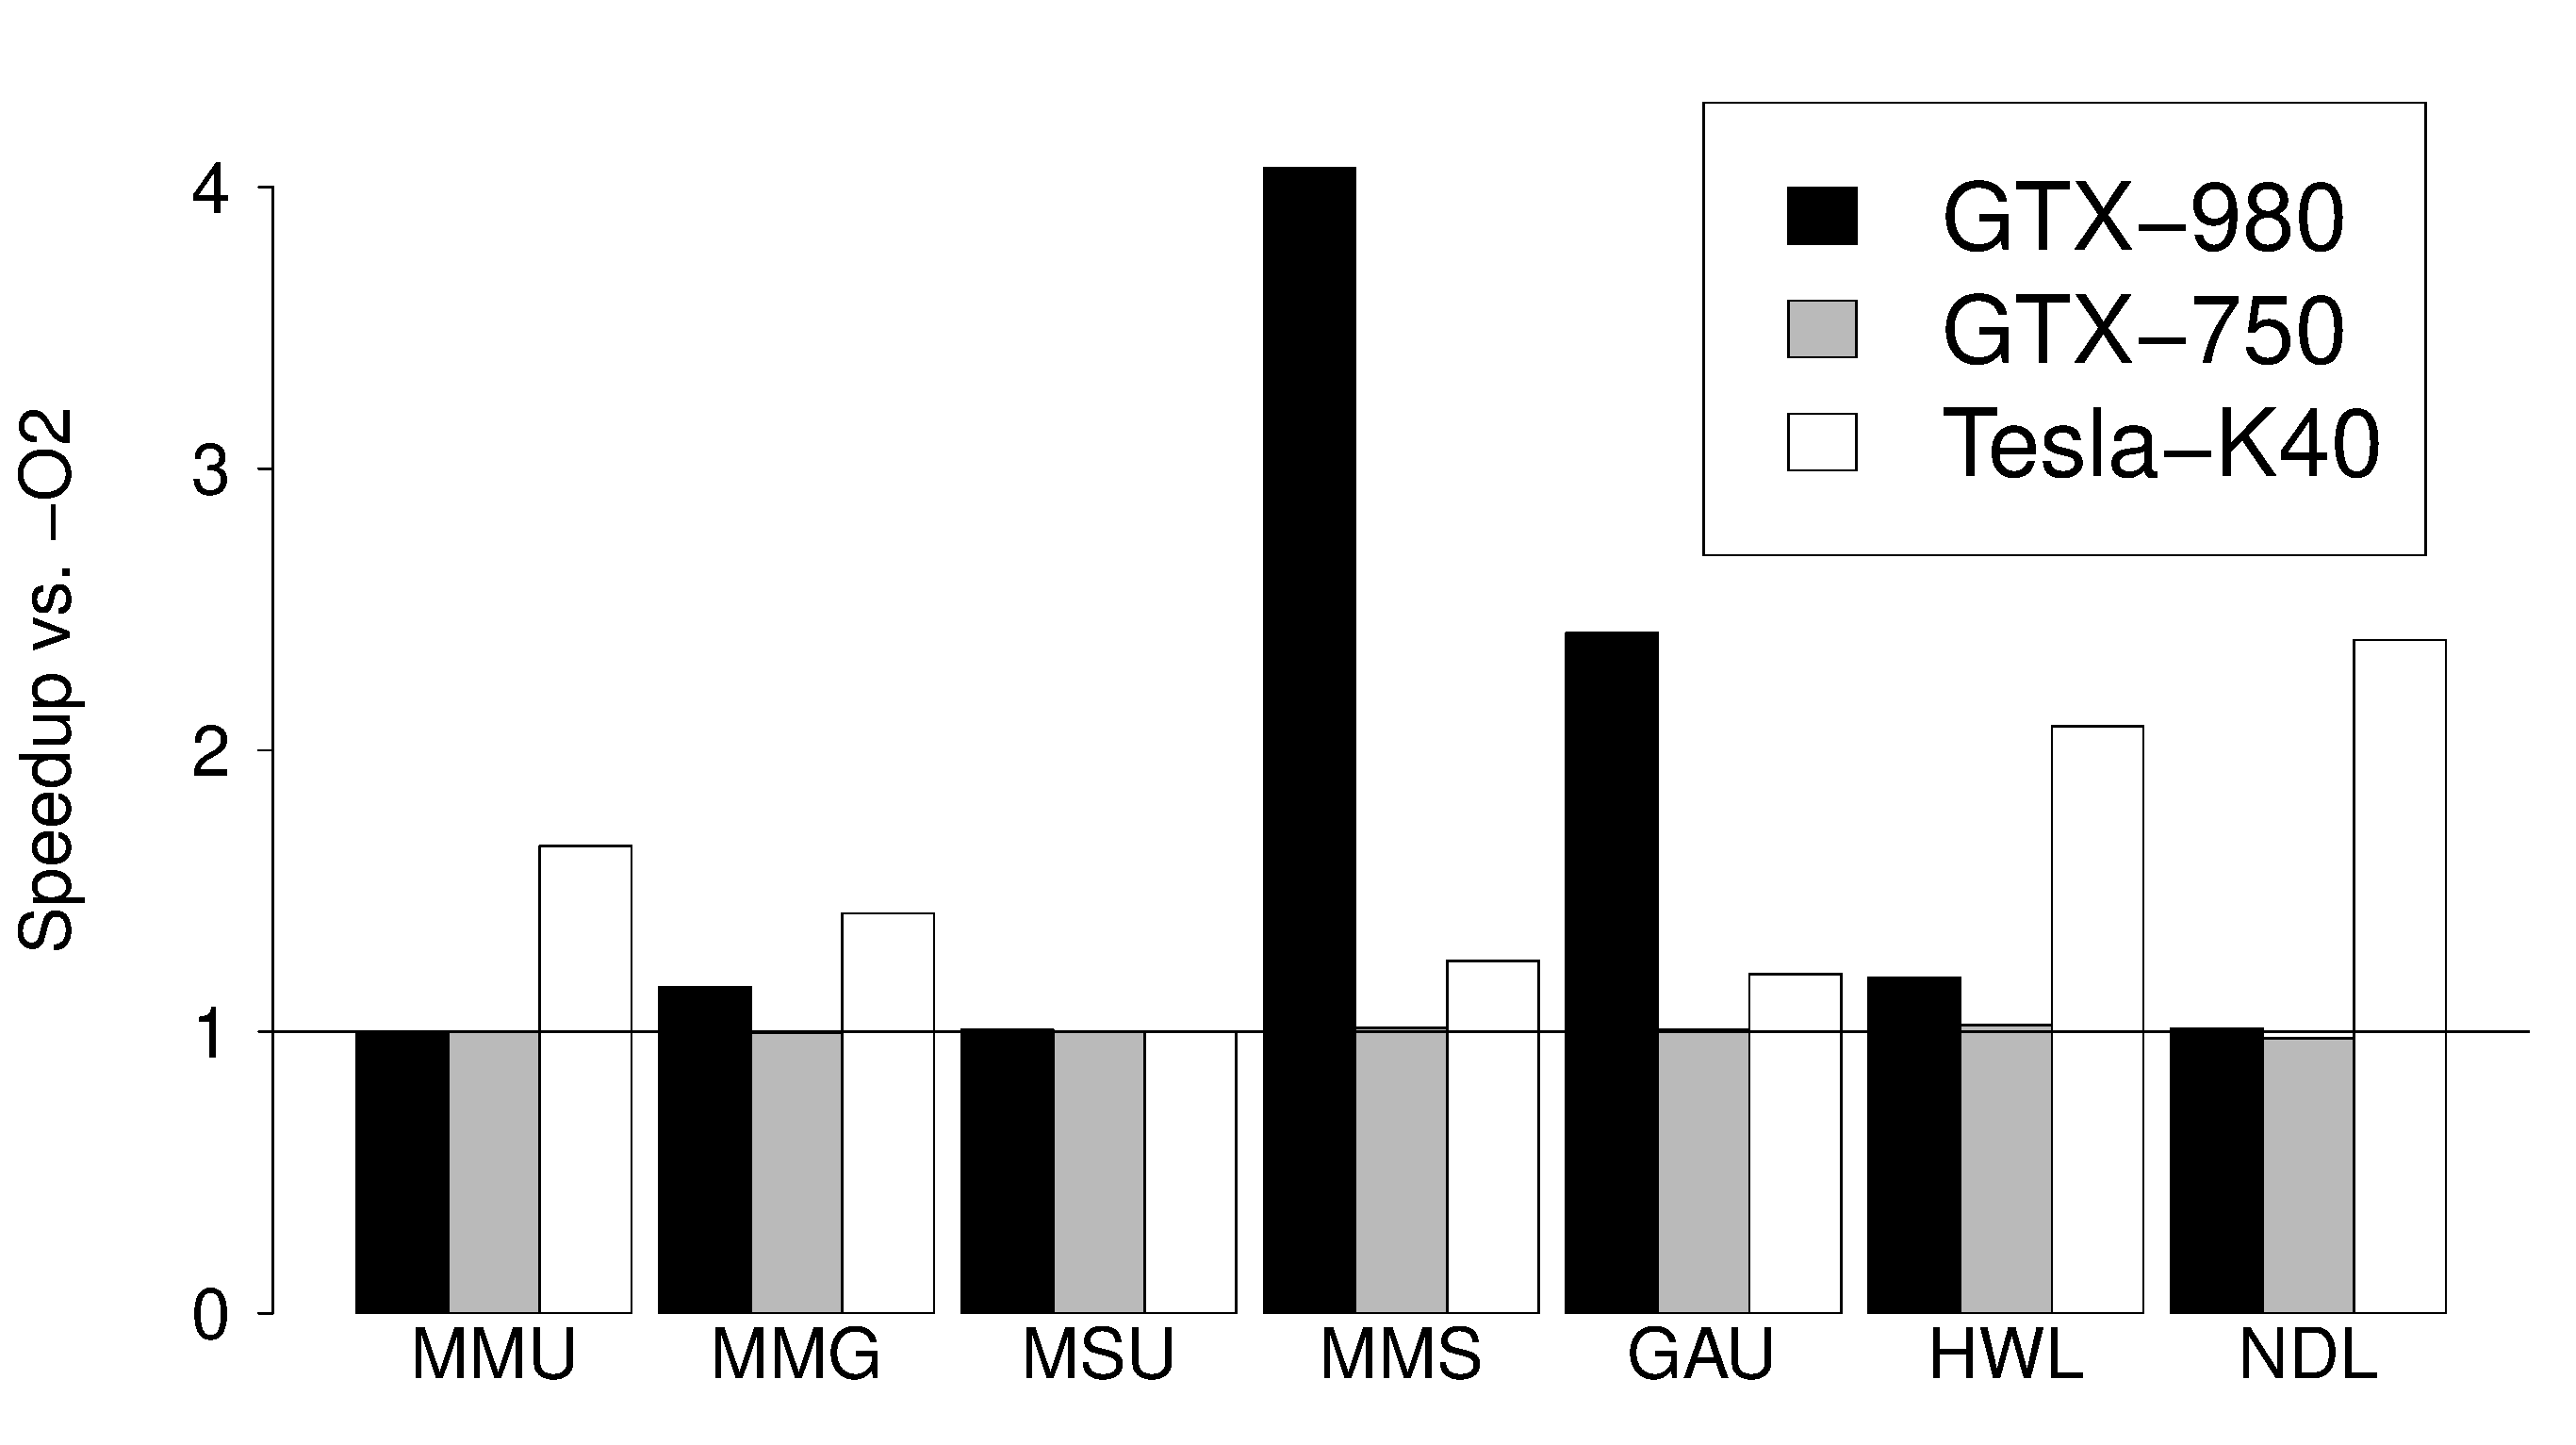
\includegraphics[width=.6\textwidth]{GPU-tuning-summary}
    \end{center}

    We \alert{found no globally good parameter selections} for specific GPUs or applications
\end{frame}

\section{Autotuning High-Level Synthesis for FPGAs}

%\begin{frame}
%    \frametitle{High-Level Synthesis for FPGAs: From C to Hardware}
%    \begin{center}
%        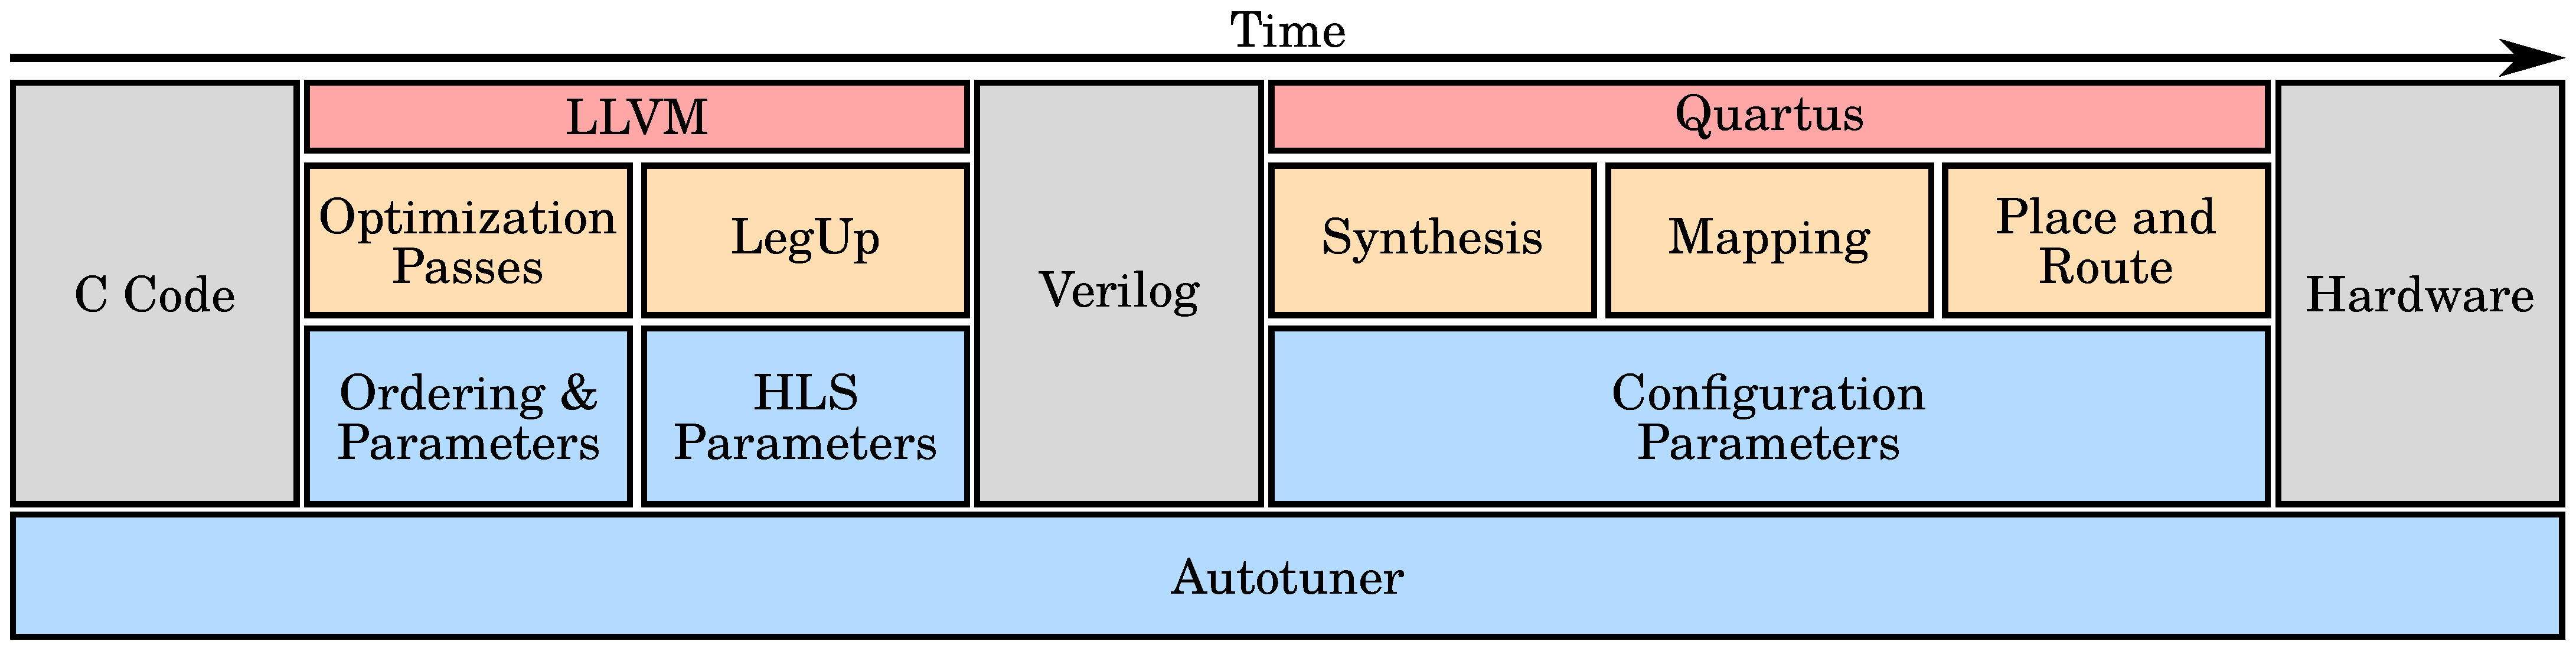
\includegraphics[width=1\textwidth]{fpga-stack-all-colors}
%    \end{center}
%
%    \begin{itemize}
%        \item We tuned applications from the \alert{CHStone Benchmark Suite}
%        \item C $\rightarrow$ Verilog: takes \alert{seconds}; \alert{\textasciitilde16\% speedup}
%        \item Verilog $\rightarrow$ Hardware: takes \alert{minutes}, \alert{hours}; \alert{10\%-2x speedup}
%        \item We tuned C $\rightarrow$ Verilog, but had \alert{to pay the cost} of Verilog $\rightarrow$ Hardware
%    \end{itemize}
%\end{frame}

\begin{frame}
    \frametitle{High-Level Synthesis for FPGAs: From C to Hardware}
    \begin{center}
        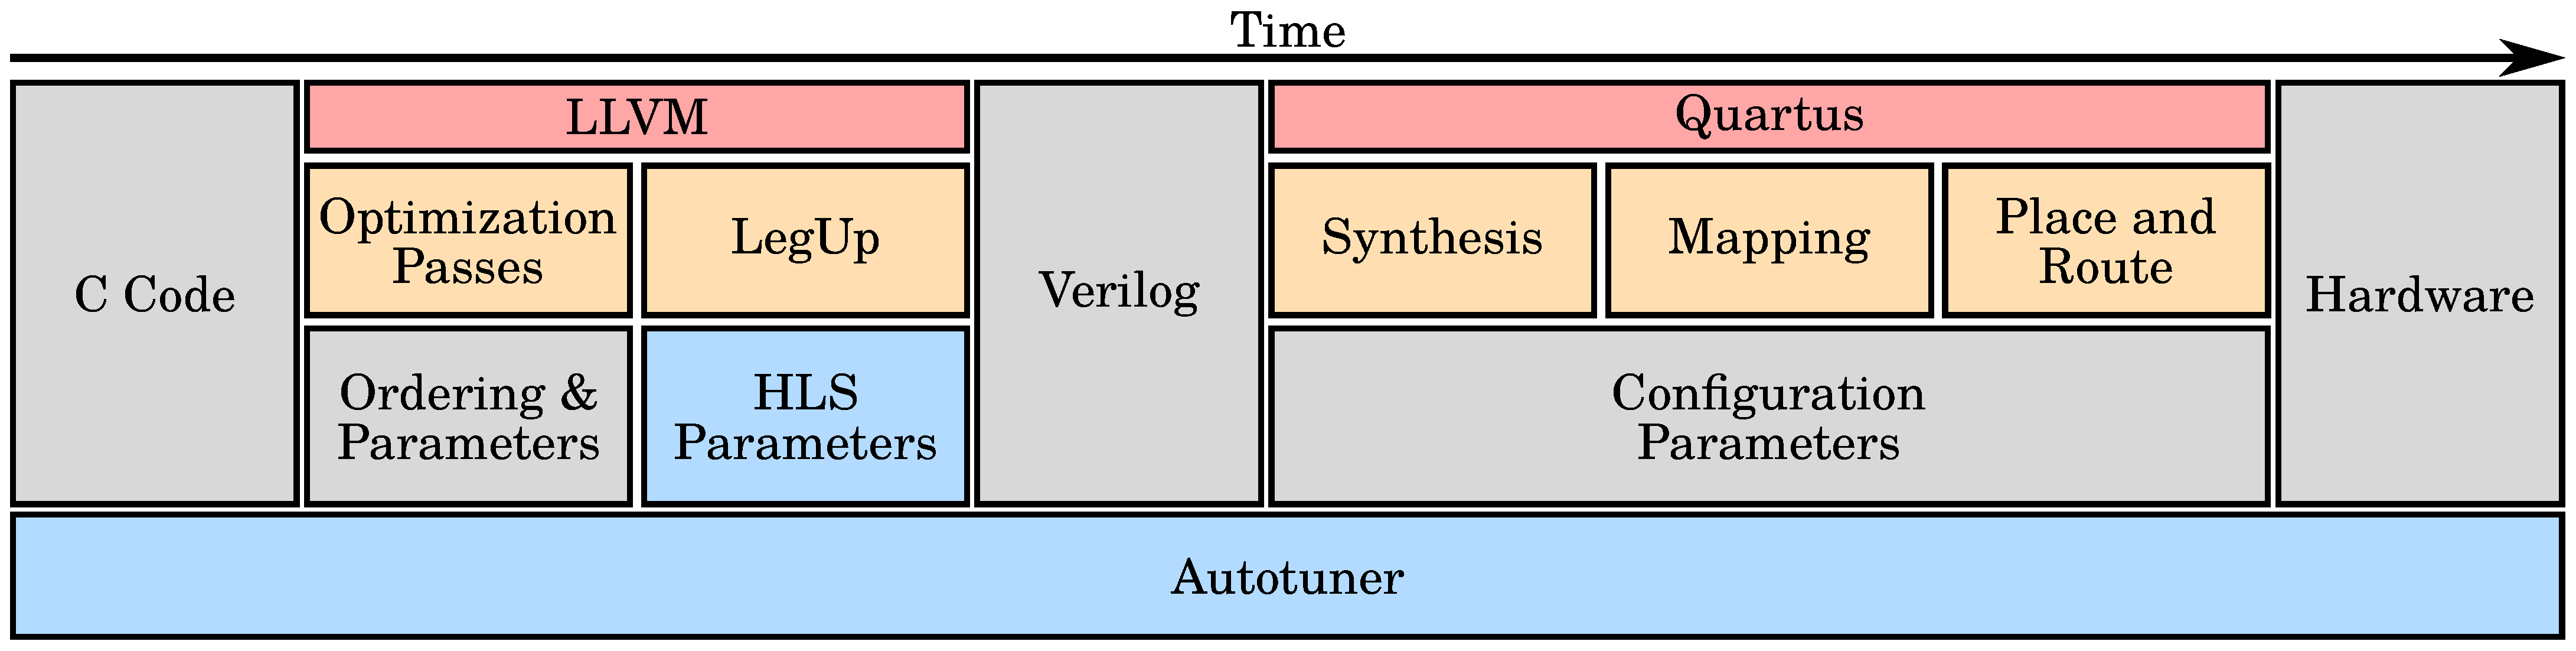
\includegraphics[width=1\textwidth]{fpga-stack}
    \end{center}

    \begin{itemize}
        \item We tuned applications from the \alert{CHStone Benchmark Suite}
        \item C $\rightarrow$ Verilog: takes \alert{seconds}; \alert{\textasciitilde16\% speedup}
        \item Verilog $\rightarrow$ Hardware: takes \alert{minutes}, \alert{hours}; \alert{10\%-2x speedup}
        \item We tuned C $\rightarrow$ Verilog, but had \alert{to pay the cost} of Verilog $\rightarrow$ Hardware
    \end{itemize}
\end{frame}

%\begin{frame}
%    \frametitle{Autotuning LegUp Parameters for CHStone}
%    \begin{center}
%        
\includegraphics[width=.73\textwidth]{overview_fpgas_small}
%
%         \alert{1h} of tuning $\rightarrow \; \dfrac{60min}{\sim{}min} \approx \alert{10}$ \alert{iterations}
%    \end{center}
%\end{frame}

%\begin{frame}
%    \frametitle{Autotuning LegUp Parameters for CHStone}
%    \alert{Search Space}:
%    \begin{itemize}
%        \item \alert{LegUp constraints} that impact \alert{Verilog generation}
%        \item Read from a \alert{configuration file}
%    \end{itemize}
%
%    Examples:
%    \begin{itemize}
%        \item \texttt{set\_accelerator\_function}
%        \item \texttt{ENABLE\_PATTERN\_SHARING}
%    \end{itemize}
%
%    \begin{center}
%        \tiny{Source: \url{legup.eecg.utoronto.ca/docs/4.0/constraintsmanual.html\#constraints} [Accessed on 15/09/16]}
%    \end{center}
%\end{frame}
%
%\begin{frame}
%    \frametitle{Autotuning LegUp Parameters for CHStone}
%    Calculating the \alert{fitness function}:
%
%    \begin{itemize}
%        \item $M$: the set of \alert{metrics}
%        \item $W$: the set of \alert{weights for each metric}
%        \item $m_{i}^{0}$: \alert{initial measured value} for each metric
%        \item $f(M,W)$: \alert{cost} or \alert{fitness function}, defined as
%    \end{itemize}
%    \begin{align*}
%        f(M, W) = \dfrac{\sum\limits_{\substack{m_i \in M \\ w_i \in W}}{w_i\Big(\dfrac{m_i}{m_{i}^{0}}\Big)}}{\sum\limits_{w_i \in W}{w_i}}
%    \end{align*}
%    \begin{itemize}
%        \item \alert{Naive weights}: $w_i = 1, \; \forall w_i \in W$
%    \end{itemize}
%\end{frame}

\begin{frame}
    \frametitle{Results for Different Optimization Scenarios}
    Decreases for the \alert{Weighted Normalized Sum} of
    hardware metrics in \alert{4 optimization scenarios}, mean of \alert{10
    tuning runs} of \alert{1.5h each}, for the \alert{StratixV DE5} FPGA:

    \begin{center}
        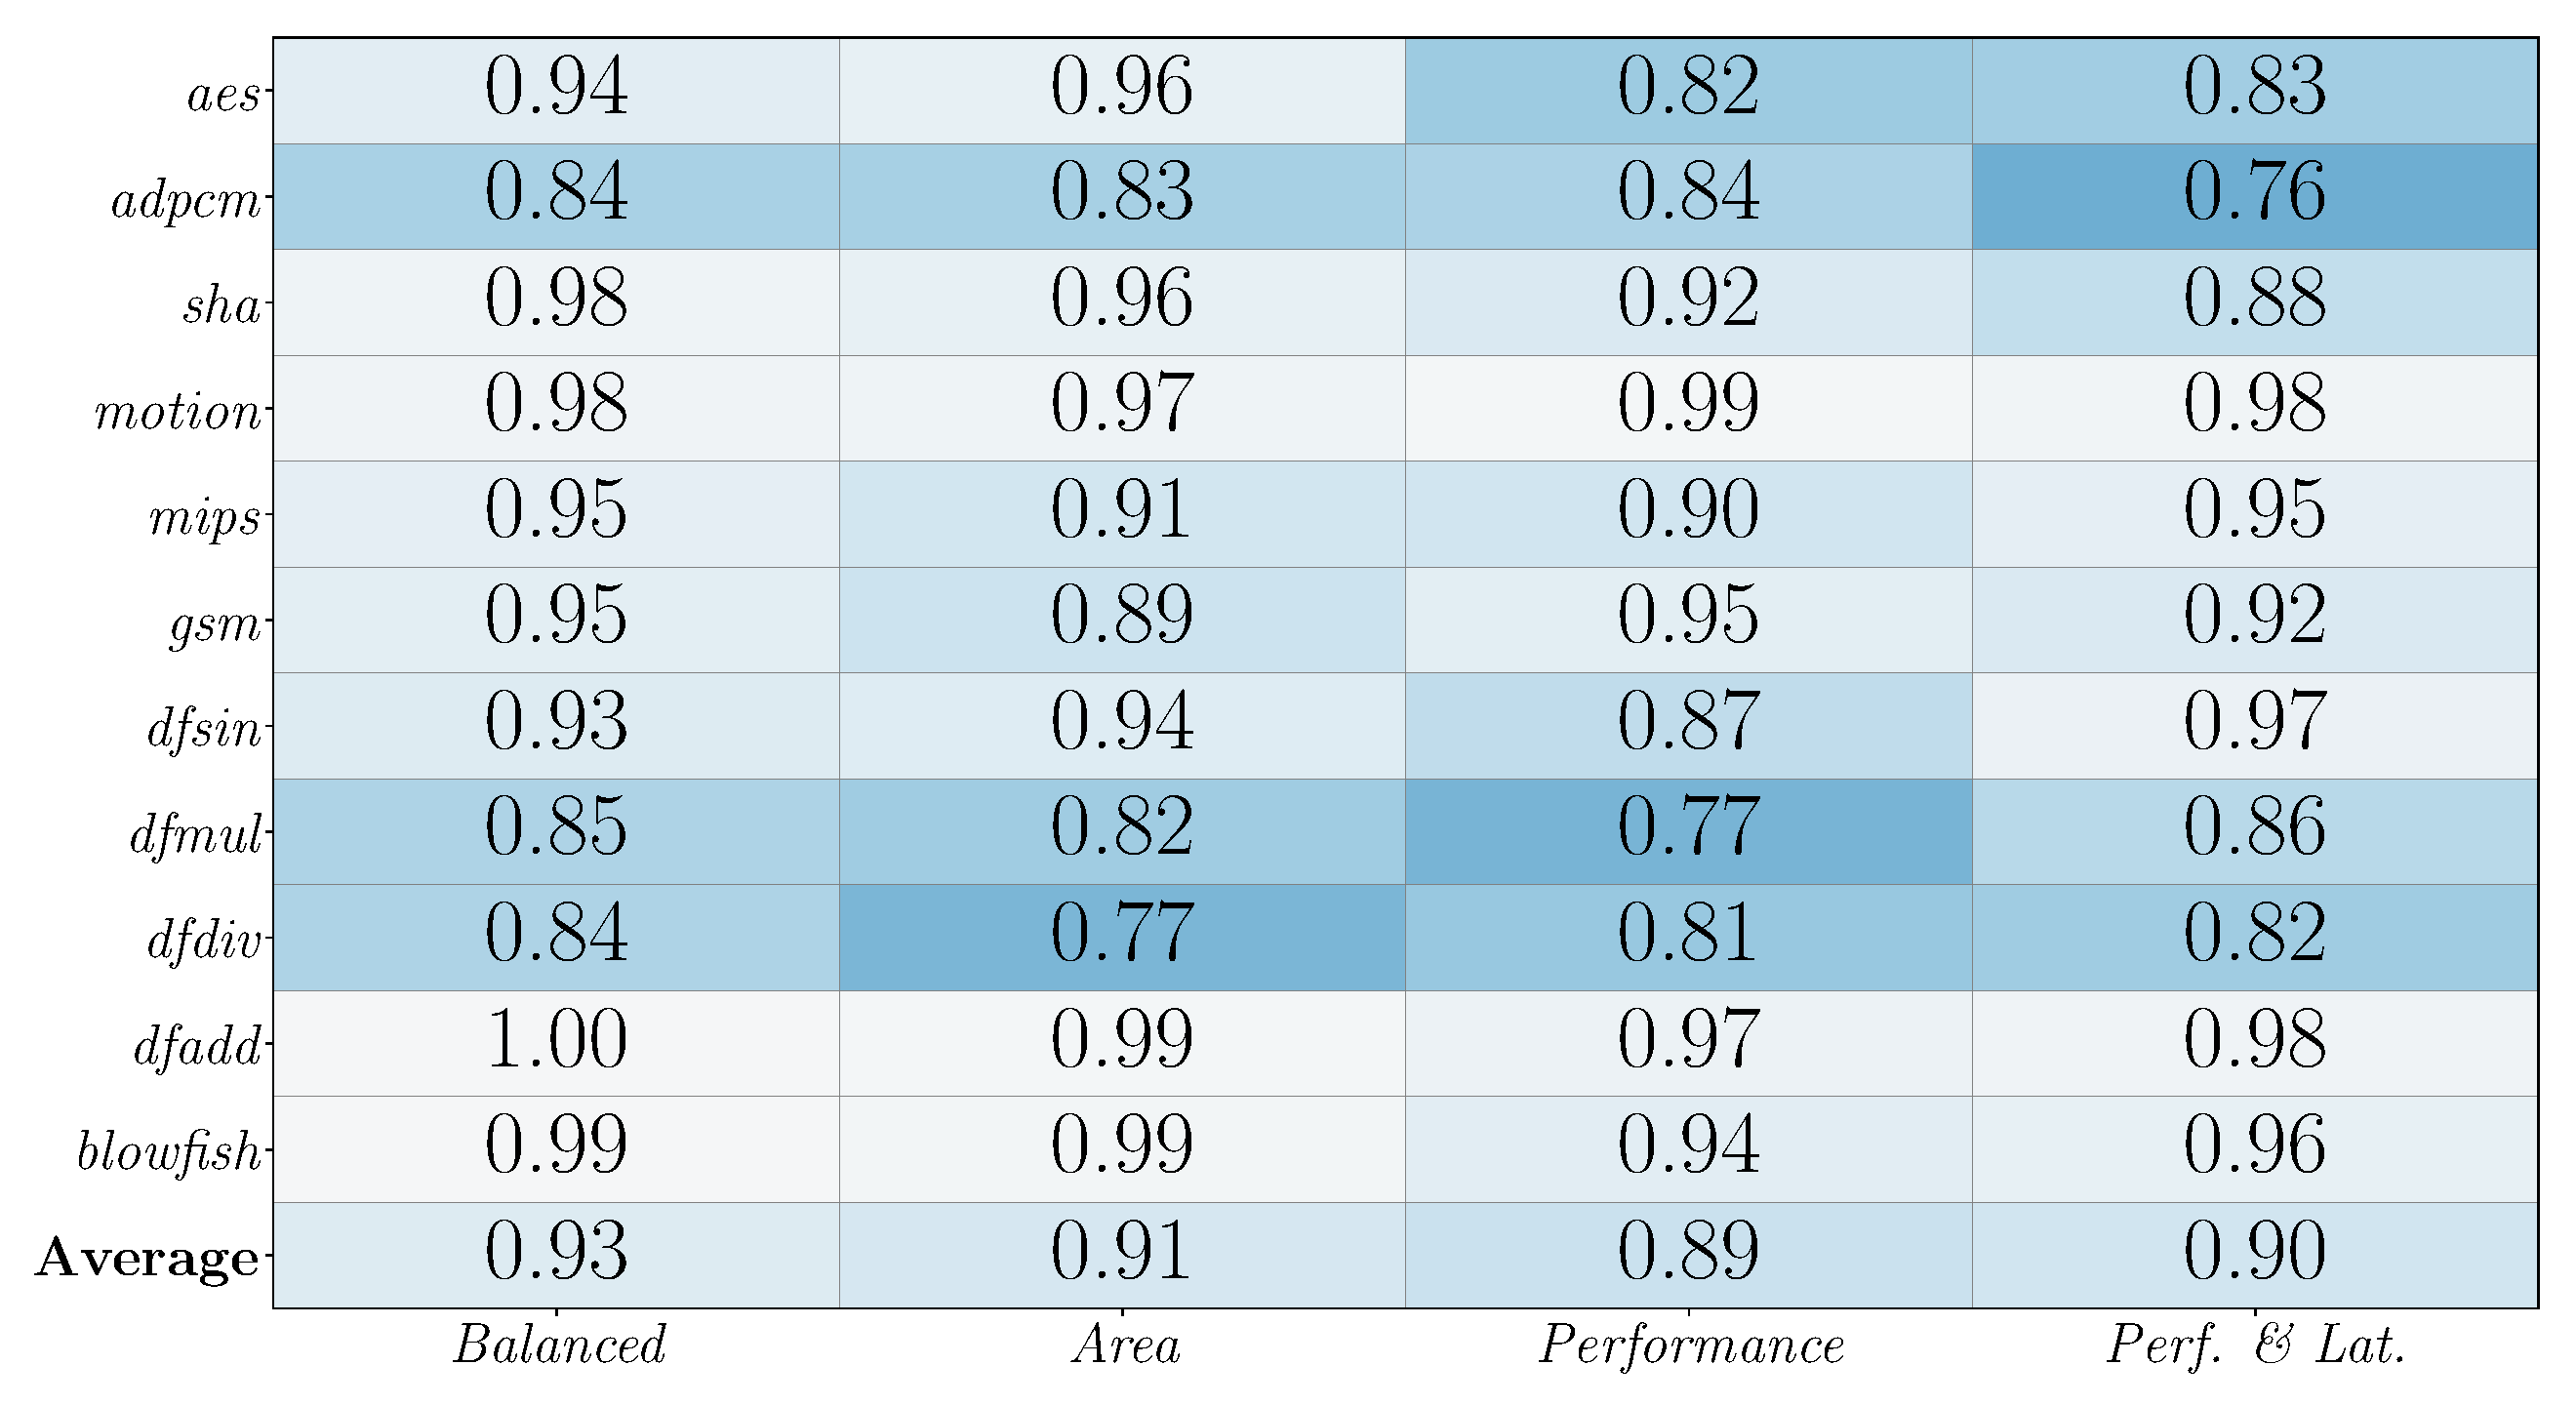
\includegraphics[width=0.8\textwidth]{heatmap_wns_comparison}
    \end{center}
\end{frame}

%\begin{frame}
%    \frametitle{Next Steps: Expensive-to-Evaluate Functions}
%    \begin{center}
%        
\includegraphics[width=.73\textwidth]{overview_fpgas_big}
%    \end{center}
%
%    \begin{itemize}
%        \item \alert{1h} of tuning $\rightarrow \; \dfrac{1h}{\sim{}h} \approx \alert{1}$ \alert{iteration}
%        \item Iterations now \alert{take too long}
%    \end{itemize}
%\end{frame}

\begin{frame}
    \frametitle{Next Steps: Autotuning for the DPE}
    Autotuning \alert{hardware and software} in the context of the DPE:

    \begin{columns}[T,onlytextwidth]
        \column{0.5\textwidth}
        \alert{Hardware search space}:
        \begin{itemize}
            \item ADC Configuration
            \item Communication between tiles
            \item Number of crossbars, IMAs in tiles
            \item Size of DPE, routing tables, eDRAM buffers
            \item $\dots$
        \end{itemize}

        \alert{DPE metrics}:
        \begin{itemize}
            \item Usability
            \item Bandwidth, Latency, Throughput
            \item Computation and Power Efficiency
            \item $\dots$
        \end{itemize}

        \column{0.5\textwidth}
        \alert{Software search space}:
        \begin{itemize}
            \item ADC usage
            \item Tile usage
            \item Mapping to memristor arrays, layers, routing tables
            \item $\dots$
        \end{itemize}

        \alert{Measurement using models}:
        \begin{itemize}
            \item Area and power overhead for components
            \item Cycle accurate simulations for accessing eDRAM, communicating tiles
            \item $\dots$
        \end{itemize}
    \end{columns}

    \vfill
\end{frame}

\begin{frame}
    \frametitle{Next Steps: Parallel and Distributed Autotuning}
    \begin{center}
        
\includegraphics[width=.3\textwidth]{stochasticsearch_logo}
    \end{center}

    We are working on an autotuning framework:
    \begin{itemize}
        \item In the \alert{Julia} language
        \item High-Level abstractions
        \item \alert{Parallel and distributed autotuning}
        \item \alert{Expensive-to-evaluate functions}
        \item \url{github.com/phrb/StochasticSearch.jl}
    \end{itemize}
\end{frame}

%\maketitle

\end{document}
